\section{Results: Context Dependence and Decision Limits}\label{sec:results}
\subsection{Static proxies: useful but not universal}
Table~\ref{tab:static-validation} reports the saved associations with positive isolated \emph{loss} damage. The gradients carry information on these balanced candidate sets, but the intervals are not pairwise tests of estimator superiority. ToyCar's target here is reconstruction MSE, not AUC. A useful MSE ranking need not protect anomaly-score ordering.
\begin{table}[t]
\caption{Sample-limited Spearman association on 320 stratified candidates per model. Intervals resample within recorded strata. Random is one saved seeded draw. Recorded runtime zeros for arithmetic/random baselines do not imply zero cost; S5/S6 share gradient computation and their rows must not be added.}\label{tab:static-validation}
\centering\small
\begin{tabular}{llrrr}\toprule
Model/loss&Score&$\rho$&Sample-design 95\% interval&Seconds\\\midrule
\csname @@input\endcsname tables/static_rank_validation.tex 
\bottomrule\end{tabular}
\end{table}

The static protection contrasts at BER .01 in Table~\ref{tab:static-protection} show why isolated predictive association is insufficient. S5 improves ResNet accuracy relative to corrected MSB in this recorded condition, whereas KWS effects are much smaller and ToyCar results depend on budget. These are task-specific effects, not evidence of a common architectural mechanism. Both interior budgets are retained rather than choosing the favorable one. All BERs and paired comparisons remain in the evidence supplement.
\begin{table}[t]
\caption{Saved paired S5-minus-MSB task-metric effects at logical BER .01. Positive favors S5. ResNet/KWS values are accuracy fractions; ToyCar values are AUC differences. Holm values retain each source's within-BER/metric family. This retrospective table is not a new confirmatory family.}\label{tab:static-protection}
\centering\small
\begin{tabular}{lrrrrr}\toprule
Model&Coverage&Fields&Effect&95\% paired interval&Holm $p$\\\midrule
\csname @@input\endcsname tables/static_comparison.tex 
\bottomrule\end{tabular}
\end{table}

\subsection{FKeras: verified numerical distinctions, limited efficacy evidence}
The KWS engineering eigensolve uses two calibration clips and two eigenpairs. Eigenvalues are approximately 5341.9031 and 434.7146, with normalized residuals $3.27\times10^{-16}$ and $3.04\times10^{-12}$, orthogonality error $6.87\times10^{-16}$, and 25 Hessian-vector products. These validate the continuous calculation, not Taylor accuracy for large encoded faults. Finite-difference checks pass in sufficiently small ReLU-stable neighborhoods; coarser steps crossing gates do not pass.

Actual masks differ between paper and repository forms at partial tiers (Table~\ref{tab:fkeras}), but coincide at complete tiers. The bounded matched protection check uses two fields and four test clips; every method retains accuracy 1.0, while CE varies and beneficial perturbations are retained. It cannot establish Hessian ranking superiority. Saved construction times are approximately 0.354 seconds for S4, 3.562 shared seconds for S5/S6, and 1.125 shared seconds for the FKeras variants. The saved coordinator elapsed time is 61.48 seconds, including loading and orchestration outside the timed score calculations. These setup-dominated measurements are not scalable throughput claims.
\begin{table}[t]
\caption{Exact symmetric differences between full KWS protection masks in the FKeras engineering check. Paper/repository differ by 901 exchanged positions at partial tiers. Equal masks under paired fields must give equal results.}\label{tab:fkeras}
\centering\small
\begin{tabular}{rrrrr}\toprule
Coverage&Protected bits&Paper/repository&MSB/paper&MSB/repository\\\midrule
\csname @@input\endcsname tables/fkeras_masks.tex 
\bottomrule\end{tabular}
\end{table}

\subsection{Exact conditional effects and the exploratory frozen pool}
M9.5.2 directly changes the background while retaining each bit identity. At $p=0$, conditional and isolated effects agree. At positive BER, point orderings change in both sample partitions (Table~\ref{tab:conditional-ranks}). These reversals share candidates and fields and are not independent binomial trials. Figure~\ref{fig:conditional} shows all ten held-out candidates rather than only a sign-changing example.
\begin{table}[t]
\caption{M9.5.2 exact isolated versus estimated conditional ordering for ten explicit KWS bits. Train/test use 64/128 fields and 256/512 clips. Spearman concerns these ten bits only.}\label{tab:conditional-ranks}
\centering\small
\begin{tabular}{lrrr}\toprule
Split&BER&Strict reversals/comparable pairs&Spearman\\\midrule
\csname @@input\endcsname tables/conditional_ranks.tex 
\bottomrule\end{tabular}
\end{table}
\begin{figure}[t]
\centering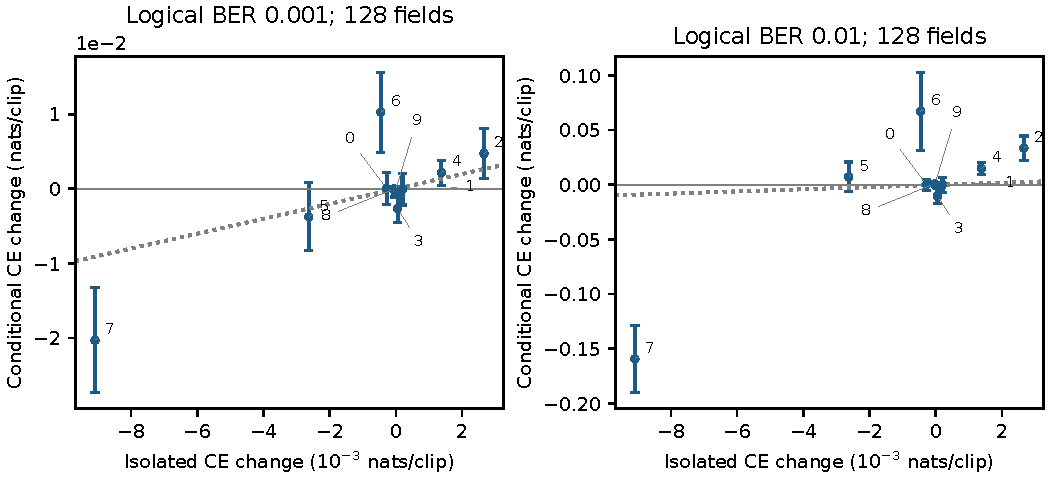
\includegraphics[width=\linewidth]{conditional_damage.pdf}
\caption{Exact isolated CE change versus mean conditional change, M9.5.2. Vertical bars are marginal field-level 95\% intervals conditional on the fixed 512 clips. Numbers index the same ten frozen candidates across panels. Beneficial and harmful changes remain signed; intervals are not adjusted for selecting a favorable bit.}\label{fig:conditional}
\Description{Two panels show all ten exact isolated effects and conditional means at BER .001 and .01 with error bars; the equality line does not describe many of the observations.}
\end{figure}

M9.5.7 independently evaluates previously frozen masks in one exploratory eight-bit pool. Selected, exact-isolated and original S5 masks protect local indices $(2,6)$, $(2,7)$ and $(6,7)$ respectively, with a global budget of 22,016 bits. Table~\ref{tab:replication} reports the positive evidence without treating the chosen pool as representative. The selected-versus-isolated secondary Holm value is $1.70\times10^{-28}$ under the saved paired-$t$ procedure. The mean CE benefit is small in absolute units. The selected-minus-S5 median is about $-1.80\times10^{-4}$, and eight of 256 fields are adverse; every field is retained. This result establishes a fixed-mask contrast under that protocol, not a population-wide ranking advantage.
\begin{table}[t]
\caption{M9.5.7 exploratory frozen-mask replication: 256 paired master fields, 256 fixed clips, BER .01. Negative CE favors the left method. Intervals are marginal field-level 95\% $t$ intervals, not pool-population intervals.}\label{tab:replication}
\centering\small
\begin{tabular}{lrrr}\toprule
Contrast&Mean CE difference&95\% interval&Favorable fields\\\midrule
\csname @@input\endcsname tables/frozen_replication.tex 
\bottomrule\end{tabular}
\end{table}

\subsection{All-pool independent evaluation does not resolve isolated-oracle superiority}
Table~\ref{tab:heldout} and Fig.~\ref{fig:heldout} retain all six completed campaign/BER arms. Selected-minus-S5 means are negative for all KWS arms. The more demanding selected-minus-exact-isolated marginal intervals span zero in \emph{every} arm. ResNet and ToyCar even have positive selected-minus-isolated means. These findings do not establish equality; they show that superiority is unresolved at the available sampling budgets.
\begin{table}[t]
\caption{Independent final target-minus-baseline risk for the restricted-selected mask. Equal-pool means and marginal 95\% pool-$t$ intervals; negative favors selected. CE and $1-\AUC$ retain separate units. All masks, including coincidences, remain included.}\label{tab:heldout}
\centering\small
\begin{tabular}{lllrll}\toprule
Campaign&BER&Baseline&Pools&Mean risk difference&95\% interval\\\midrule
\csname @@input\endcsname tables/heldout.tex 
\bottomrule\end{tabular}
\end{table}
\begin{figure}[t]
\centering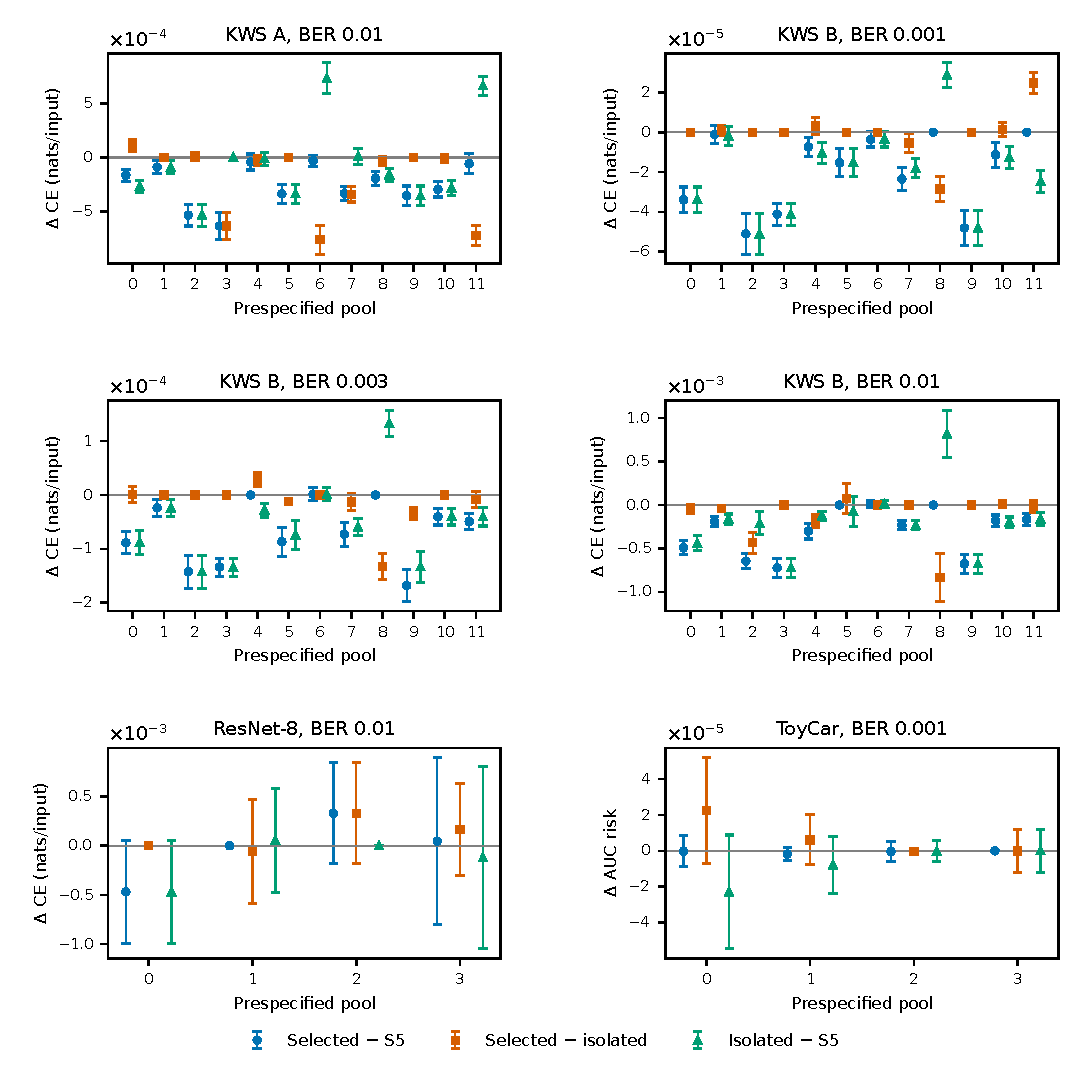
\includegraphics[width=\linewidth]{heldout_pool_effects_paper.pdf}
\caption{All finalized M9.10 held-out pool contrasts with saved marginal paired-field 95\% intervals; equal-pool intervals are in Table~\ref{tab:heldout}, not this plot. Panels retain distinct risk units and scales. The recurring twelve KWS pools do not create new independent pools at each BER.}\label{fig:heldout}
\Description{Six panels display all held-out paired mask effects and field-level intervals, including zero and adverse cases.}
\end{figure}

The exploratory eight-bit result and these six-bit campaigns answer different questions: the first fixes a historically informed pool; the latter sample pools within source-mask status strata. Different cohorts and field counts also intervene. Selecting favorable later pools to reproduce the earlier result would invalidate the generalization question. No such filtering is used.

\subsection{Outside conditioning dominates recorded selection reordering}
The exact signed decomposition closes to a maximum absolute residual of $3.55\times10^{-15}$ across recorded fields and masks. Clean isolated predictions produce many strict mask-order reversals, while background-conditioned singleton predictions produce few (Table~\ref{tab:reversals}). The latter can still miss nonzero interactions; decision contributions are weighted by $p^2,p^3,\ldots$ and need not reflect the size of forced multi-bit effects.
\begin{table}[t]
\caption{Selection-mask order reversals against exact candidate integration. Denominators count strict comparable pairs after a diagnostic $10^{-12}$ near-tie exclusion; pairs are not independent observations. No mask is changed by the diagnostic threshold.}\label{tab:reversals}
\centering\small
\begin{tabular}{llrr}\toprule
Campaign&BER&Clean isolated&Outside-conditioned\\\midrule
\csname @@input\endcsname tables/reversals.tex 
\bottomrule\end{tabular}
\end{table}
\begin{table}[t]
\caption{Signed selection-data selected-minus-isolated attribution, equally averaged over all pools. The first three columns sum to the last. CE units apply except ToyCar, which is $1-\AUC$. These are post-selection descriptive contrasts, not unbiased held-out gains.}\label{tab:attribution}
\centering\small
\begin{tabular}{llllll}\toprule
Campaign&BER&Clean&Outside&Within candidate&Exact\\\midrule
\csname @@input\endcsname tables/attribution.tex 
\bottomrule\end{tabular}
\end{table}

Crucially, these are model-selection tables. The final paired-swap archive lacks complete final subcubes and matching same-final-cohort clean-isolated controls. We therefore cannot attribute a final risk contrast to these three components, nor assign selection/final disagreement uniquely to interaction, input shift, or field noise.

\subsection{ToyCar: real interactions, coarse cohorts, unresolved decisions}
The clean selection and final AUCs are 0.826389 and 0.920139 on balanced 24- and 48-file cohorts. One untied pair reversal changes their AUC by $1/144$ and $1/576$; ties receive half credit. This is single-state metric resolution, not a floor on expected differences, which may be much smaller after multiplication by $p$ and averaging.

Across the four pools, 390, 296, 332 and 288 of 504 nonempty forced candidate-state responses change AUC relative to their field's empty candidate state. These states are not equiprobable Bernoulli outcomes. Mean outside-field risks are roughly .45, .39, .44 and .44, showing substantial degradation despite tiny mask contrasts. The selected and original masks coincide in one pool, yielding a structurally zero selected-minus-S5 contrast there; other pools contain nonzero field effects. Neither the unresolved aggregate result nor small expected corrections imply an absence of interactions.
\begin{figure}[t]
\centering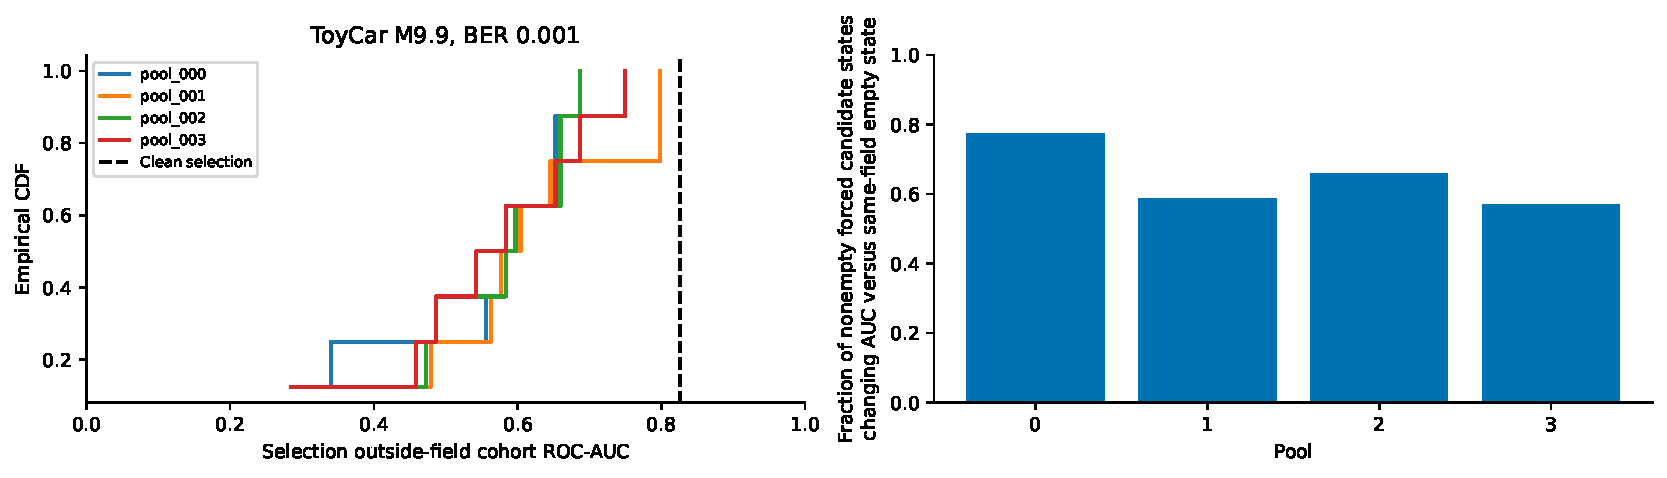
\includegraphics[width=\linewidth]{toycar_resolution.pdf}
\caption{Finalized complete-file ToyCar diagnostics: cohort metric resolution, background degradation and changes under forced candidate states. Forced states are diagnostics, not uniformly weighted deployment events. No window-wise AUC or additive file-loss substitution is made.}\label{fig:toycar}
\Description{ToyCar panels display clean and faulted cohort risks and how frequently forced candidate states change AUC, despite small expected protection contrasts.}
\end{figure}

\subsection{M11: approximation validation is not a large-scale efficacy result}
Reusing the 56 recorded exact pool/BER tables requires no new inference. Table~\ref{tab:approximation} shows that the outside-additive choice attains the recorded finite-field optimum in the classification arms, while ToyCar's mean finite-field regret is approximately $2.17\times10^{-10}$. This near-agreement is meaningful for these small low-occupancy candidate pools, not a certificate for larger pools, unseen fields or the final task population.
\begin{table}[t]
\caption{M11 offline reuse of all historical exact selection tables. Error is the pool-mean of maximum absolute mask-risk error; regrets compare choices on those same finite selection fields. These are not independent final performance estimates.}\label{tab:approximation}
\centering\small
\begin{tabular}{lllll}\toprule
Campaign&BER&Outside max error&Outside regret&Clean regret\\\midrule
\csname @@input\endcsname tables/approximation.tex 
\bottomrule\end{tabular}
\end{table}

Separate engineering checks use two previously exposed inputs (complete files for ToyCar), BER .003, and only one or two outside fields. KWS $K=8$ produces nonzero outside-additive regret, while $K=12$ has many strict ordering reversals but zero decision regret on the recorded field (Table~\ref{tab:oracle}). Ranking agreement and decision quality are therefore different objectives. Small ToyCar checks are especially coarse. No large-$K$ optimum or broad protection advantage was measured.
\begin{table}[t]
\caption{Bounded M11 outside-additive versus exact oracle checks, not publication efficacy trials. Times are recorded evaluation work including controls, excluding process startup. Each cohort has only two inputs/files.}\label{tab:oracle}
\centering\small
\begin{tabular}{lrrllrr}\toprule
Model&$K$&Fields&Max error&Selection regret&Reversals&Seconds\\\midrule
\csname @@input\endcsname tables/oracle.tex 
\bottomrule\end{tabular}
\end{table}

The formal bound is conservative here. For $K=6,r=2,p=.01$ and clipped classification CE, $\epsilon_m=0.03283$ nats, far larger than the recorded outside-additive errors and many final decision effects. ToyCar at $p=.001$ has $\epsilon_m\approx1.20\times10^{-5}$. Finite-field uncertainty increases the certificate further. The bound is useful for identifying assumptions and failure regimes; it does not statistically resolve the observed small differences.

\subsection{Computational cost}
Each $K=6$ selection field requires 64 cohort states and yields all 15 legal mask risks. The outside-singleton approximation needs seven states per field, but selecting well with it may still require many fields. At $K=8$ and 12 the corresponding reference/approximation counts are 256/9 and 4096/13. These are exact operation ratios, not measured end-to-end speedups.
\begin{table}[t]
\caption{Saved engine wall times summed across pools, in seconds. Setup is included. Concurrent campaign elapsed time and machine-independent throughput cannot be inferred from these sums.}\label{tab:costs}
\centering\small
\begin{tabular}{llrr}\toprule
Campaign&BER&Selection&Final\\\midrule
\csname @@input\endcsname tables/costs.tex 
\bottomrule\end{tabular}
\end{table}
A ToyCar cohort state evaluates every window of every complete file: 24 selection files imply 4,704 window inferences per state. The finalized M9.10 replay uses saved responses with no model calls. Costs and decision magnitudes must be considered together; response-table reuse saves new inference but cannot create information about unobserved final states.
\FloatBarrier
